%!TEX root = ./main.tex


\tikzset{every picture/.style={line width=0.75pt}} %set default line width to 0.75pt        

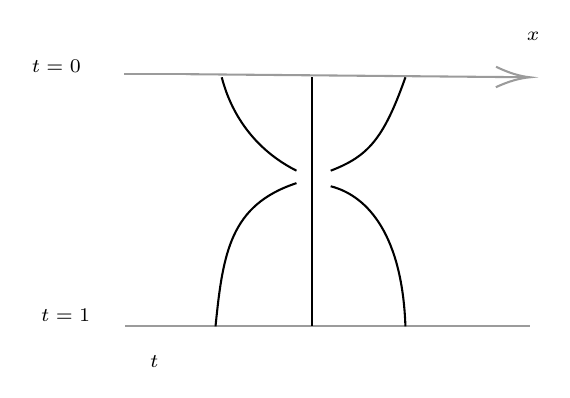
\begin{tikzpicture}[x=0.75pt,y=0.75pt,yscale=-1.5,xscale=1.5]
%uncomment if require: \path (0,300); %set diagram left start at 0, and has height of 300

%Straight Lines [id:da9999252093097876] 
\draw [color={rgb, 255:red, 155; green, 155; blue, 155 }  ,draw opacity=1 ]   (209.5,69) -- (318,69.98) ;
\draw [shift={(320,70)}, rotate = 180.52] [color={rgb, 255:red, 155; green, 155; blue, 155 }  ,draw opacity=1 ][line width=0.75]    (10.93,-3.29) .. controls (6.95,-1.4) and (3.31,-0.3) .. (0,0) .. controls (3.31,0.3) and (6.95,1.4) .. (10.93,3.29)   ;
%Straight Lines [id:da8602700993161204] 
\draw [color={rgb, 255:red, 155; green, 155; blue, 155 }  ,draw opacity=1 ]   (209.5,69) -- (189.5,69) ;
%Straight Lines [id:da31711673101036175] 
\draw [color={rgb, 255:red, 155; green, 155; blue, 155 }  ,draw opacity=1 ]   (320,150) -- (190,150) ;
%Straight Lines [id:da02070104769775316] 
\draw    (250,70) -- (250,150) ;
%Curve Lines [id:da05791226204824307] 
\draw    (221,70) .. controls (222.4,75.4) and (227.2,91) .. (245,100) ;
%Curve Lines [id:da40088925285683386] 
\draw    (280,70) .. controls (273,89.8) and (268,95.4) .. (256,100) ;
%Curve Lines [id:da876049615716019] 
\draw    (219,150) .. controls (221.4,126.2) and (223.8,111) .. (245,104) ;
%Curve Lines [id:da5837647469150872] 
\draw    (256,105) .. controls (268.4,108.2) and (279,121.4) .. (280,150) ;

% Text Node
\draw (159,63.4) node [anchor=north west][inner sep=0.75pt]  [font=\scriptsize]  {$t=0$};
% Text Node
\draw (162,143.4) node [anchor=north west][inner sep=0.75pt]  [font=\scriptsize]  {$t=1$};
% Text Node
\draw (197,158.4) node [anchor=north west][inner sep=0.75pt]  [font=\scriptsize]  {$t$};
% Text Node
\draw (318,54.4) node [anchor=north west][inner sep=0.75pt]  [font=\scriptsize]  {$x$};


\end{tikzpicture}